\chapter{Dialogflow}
	\section{What is Dialogflow?}
	\textit{Dialogflow} is a powerful NLP developed by Google, born from the \textit{API.ai} project, which aims to provide a rich conversational experience and a strong ease in using and developing the bot.\\\\
	One of the strength points of \textit{Dialogflow} is, first of all, its machine learning power: indeed, it's able to recognize complex entities inside sentences, and react also to big changes in the sentences with respect to the training ones. Another important point to notice, is the simplicity with which it can be trained: it provides a pleasant UI that lets adding intents, entities, training sentences, managing contexts and, in general, avoiding low-level details. Each of the terms we're used so far, are fundamental elements of the Dialogflow job: now we're going to see them in details.
	
	\section{How does it work?}
	First of all, the \textit{Dialogflow} natural language processing analyzes the input that the user sends thanks to a client, which can be a web platform, a messaging application, or even a device with a microphone which takes as input the user's voice.\\\\
	\textit{Dialogflow}, except for base sentences, has to retrieve some data to fulfill the user's request: this can be done thanks to a data source. It can be, of course, any possible data store, like a database, a knowledge base, etc.\\\\
	\textit{Dialogflow}, retrieved the information, has to provide an answer: it can be done with a series of methods: textual, voice, graphics. It depends on the device that the user is using to talk with the bot.
	
	\begin{figure}[H]
		\centering
		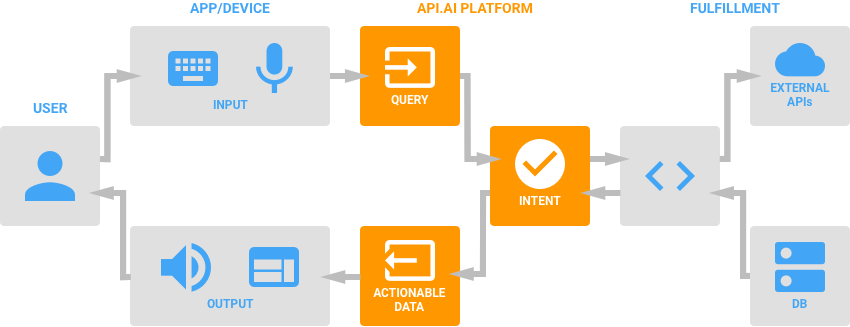
\includegraphics[scale=0.4]{apiai}
		\caption{Architecture of a generic system using \textit{Dialogflow}\cite{apiai}}
	\end{figure}
	
	\section{Fundamental concepts}
		Dialogflow works thanks to some fundamental pillars:
		\begin{itemize}
			\item \textbf{Intents}\\
			They are the mapping between the user query and the desired action. Each intent, indeed, corresponds to "what the user wants to do" in a certain fraction of the conversation.
			\item \textbf{Entities}\\
			They are fragments of natural language inputs, corresponding to a specific type. They can be cities, places, numbers, names, etc. There are a lot of default entities, but custom entities can be created by the user.
			\item \textbf{Actions}\\
			Actions represent what the bot needs to do after the intent has been resolved.
			\item \textbf{Parameters}\\
			They are all the values that are needed to perform an action.
			\item \textbf{Contexts}\\
			They are "containers" in which all the entities and parameters of the conversation are stored. They are fundamental to keep the informations through the conversational flow and make possible the "slot-filling".
		\end{itemize}
	One of the most powerful aspects of \textit{Dialogflow} is the support for slot-filling. It is a technique that lets users to specify details (necessary or not) in different phases of the conversation: this means that the bot can go ahead and keep asking more details to the user before answering the query. Let's make an example:
	
	\begin{verse}
		\textit{Please give me 2 works} - \textbf{User}\\
		\textit{You told me few filters. Do you want to add something?} - \textbf{Bot}\\
		\textit{Yes!} - \textbf{User}\\
		\textit{Ok, tell me what} - \textbf{Bot}\\
		\textit{The artist} - \textbf{User}\\
		\textit{Ok! Just tell me his name} - \textbf{Bot}\\
		\textit{Mozart} - \textbf{User}\\
		\textit{Perfect! Do you want to add something else?} - \textbf{Bot}\\
		...\\
	\end{verse}
	This result is obtained thanks to the "required" entity: in the \textit{Dialogflow} UI (and of course, in the JSON file of the intent) it's possibile to specify some fields that are required in order to consider the intent as completed. The bot will provide the final answer of the user's request if and only if all the required slot have been filled! This means that the conversation can go over and over until these informations are provided.\\\\
	The power of \textit{Dialogflow} so, is heavily based on slot-filling. It is able to keep the informations through all the flow of the conversation 
